\documentclass{beamer}
%
% Choose how your presentation looks.
%
% For more themes, color themes and font themes, see:
% http://deic.uab.es/~iblanes/beamer_gallery/index_by_theme.html
%
\mode<presentation>
{
  \usetheme{default}      % or try Darmstadt, Madrid, Warsaw, ...
  \usecolortheme{default} % or try albatross, beaver, crane, ...
  \usefonttheme{default}  % or try serif, structurebold, ...
  \setbeamertemplate{navigation symbols}{}
  \setbeamertemplate{caption}[numbered]
  \setbeamertemplate{footline}[frame number]
} 

\usepackage[english]{babel}
\usepackage[utf8x]{inputenc}

\title[2016-03-07-rootteam-hadoop]{Computing practices observed in industry}
\author{Jim Pivarski}
\institute{Princeton University -- DIANA}
\date{March 7, 2016}

\xdefinecolor{darkblue}{rgb}{0.1,0.1,0.7}

\begin{document}

\begin{frame}
  \titlepage
\end{frame}

\begin{frame}{Context}

\begin{block}{}
The commercial ``Big Data'' movement developed more or less independently of high energy physics, even though some of the same problems had to be solved.
\end{block}

\begin{block}{}
This talk is about the differences I have seen between the two communities, with an emphasis on technical choices, to aid in integration and interoperablity with ROOT.
\end{block}
\end{frame}

\begin{frame}{Language choice}
\begin{block}{Short answer}
Commercial distributed systems are usually implemented in Java, and so distributed data processing systems like Hadoop and Spark are also on the Java Virtual Machine (JVM).
\end{block}

\begin{block}{Long answer}
This is the topic I get the most questions about, so I'll break it down by project (next page).
\end{block}
\end{frame}

\begin{frame}{Language choice in projects I was involved in}
\begin{itemize}
\item Credit card company: SAS and Python ({\it pure} Python, not even Numpy).

\item Web advertising start-up: Python.

\item NASA (open source Project Matsu): Java simply because it was a new project using Hadoop and HBase. I think they ordinarily use C++ for image processing.

\item Monitoring auto traffic: real-time analysis in Storm (which is Clojure, a JVM language, but I wrote my code in Scala).

\item Auto insurance: SQL over Hadoop, using Hive and Pig. User-defined functions were in Java because Hive and Pig (and Hadoop) are Java.

\item Military project: extremely Java-centric.

\item Data science start-up: most data analyses in R, a little in Python, but the web-facing data backbone was strictly Java.
\end{itemize}
\end{frame}

\begin{frame}{Major frameworks}
\begin{block}{Apache Hadoop}
Performs map-reduce calculations. Used as a foundation for other big data frameworks because of\ldots
\begin{itemize}
\item the HDFS distributed filesystem (even variants like MapR, which don't use HDFS, provide an HDFS API),
\item suite of InputFormats that split files by logical records,
\item ZooKeeper, which coordinates job configuration and synchronization across a distributed service.
\end{itemize}
\end{block}

\begin{block}{Apache Spark}
Generalizes from map-reduce to arbitrary DAG data pipelines, optimized for iterative procedures, with an interactive prompt. May be used on any cluster manager, but usually Hadoop.
\begin{itemize}
\item User interfaces: native Scala, Java, Python (through sockets), and R (through pipes).
\end{itemize}
\end{block}
\end{frame}

\begin{frame}{Major frameworks}
\textcolor{darkblue}{Google Trends result}

(frequency of use as a search term, in ``software'' context)

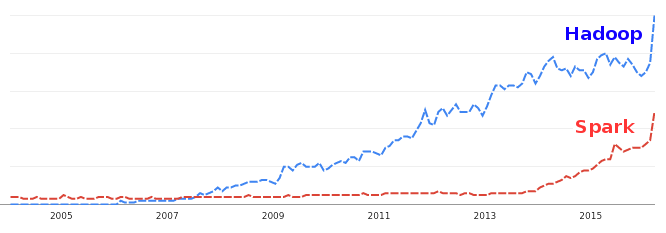
\includegraphics[width=\linewidth]{trends.png}
\end{frame}

\begin{frame}{Data pipelines and databases (frequently encountered)}

It's not uncommon to use several frameworks in a single project, whether they're orthogonal in purpose or not.

\begin{description}
\item[Apache Storm] real-time analysis, a fault-tolerant data pipeline.
\item[Apache Drill] rapid response to queries (which I think would be ideal for plotting).
\item[Apache HBase] random-access tabular database over Hadoop.
\item[Apache Hive] SQL over Hadoop ({\it not} random-access).
\item[Apache Pig] custom language (Pig Latin), ``eats any data format.''
\item[Apache Mesos] cluster manager (using ZooKeeper).
\item[Apache Kafka] message queue.
\item[Apache Flume] queues for log files.
\item[ElasticSearch] full-text search engine.
\item[MongoDB] indexable JSON document store.
\end{description}
\end{frame}

\begin{frame}{Major frameworks}
\textcolor{darkblue}{Google Trends result}

(same approximate vertical scale as before)

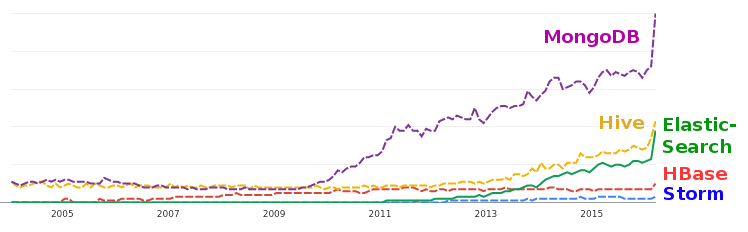
\includegraphics[width=\linewidth]{trends2.png}
\end{frame}

\begin{frame}{Generic data formats (frequently encountered)}

It's also not uncommon to mix file formats and use a lot of text-based formats. Perhaps 80\% of what I saw was JSON.

\begin{description}
\item[CSV] table of primitives: numbers, booleans, strings (text).
\item[JSON] arrays and maps of primitives (text).
\item[XML] structures with an optional schema (text).
\item[Apache Avro] JSON-like binary format with algebraic data types (arrays, maps, records, and unions of primitives). Similar to \textcolor{darkblue}{Thrift} and \textcolor{darkblue}{Protocol buffers}.
\item[Parquet] similar to Avro, but stored column-wise for speed.
\item[Sequence files] structured container of arbitrary binary blobs intended as splitting hints for Hadoop.
\item[Intermediate serialization in Hadoop and Spark] using native Java serialization, Kryo, and Hadoop Writables.
\item[Python pickle files] for persisting Python objects.
\end{description}
\end{frame}

\begin{frame}{Machine learning}
Mostly R packages, but also \textcolor{darkblue}{Mahout} (over Hadoop) and \textcolor{darkblue}{MLLib} (over Spark), and the Python numerical stack: \textcolor{darkblue}{Numpy}, \textcolor{darkblue}{SciPy}, and \textcolor{darkblue}{SciKit-Learn}.

\vfill
\hspace{-0.83 cm} \textcolor{darkblue}{\Large User interfaces}

\vspace{0.5 cm}
\textcolor{darkblue}{IPython Notebooks}, \textcolor{darkblue}{RStudio}, writing text files by hand.

\vspace{0.5 cm}
Often the only way to access the Hadoop cluster was from Citrix to a Windows VM with Putty installed to a Linux head node, which discouraged GUIs.

\vspace{0.5 cm}
Some clusters were set up with Hue, to upload job JARs through a website, but the website was only accessible through these VMs.
\end{frame}

\begin{frame}{Goals and organization}

\begin{block}{Factorization}
Hadoop is both a cluster and an analysis framework, like CRAB and CMSSW combined. Newer projects tend to be better factorized.
\end{block}

\begin{block}{Non-centralized development}
Hadoop itself is a mess:
\begin{itemize}
\item user code must be compiled against a Hadoop version,
\item the version history is complex and branches (0.23 is newer than 1.0),
\item common features like secondary sorting are actually just common user hacks\ldots
\end{itemize}

\vspace{0.2 cm}
Pretty quickly, everyone was writing layers on top of Hadoop. Just the Python ones: \textcolor{darkblue}{hadoopy}, \textcolor{darkblue}{pydoop}, \textcolor{darkblue}{mrjob}, \textcolor{darkblue}{dumbo}, \textcolor{darkblue}{luigi}, \textcolor{darkblue}{happy}, \textcolor{darkblue}{hipy}, I wrote one\ldots
\end{block}
\end{frame}

\begin{frame}{Helpful guide to Hadoop version control}
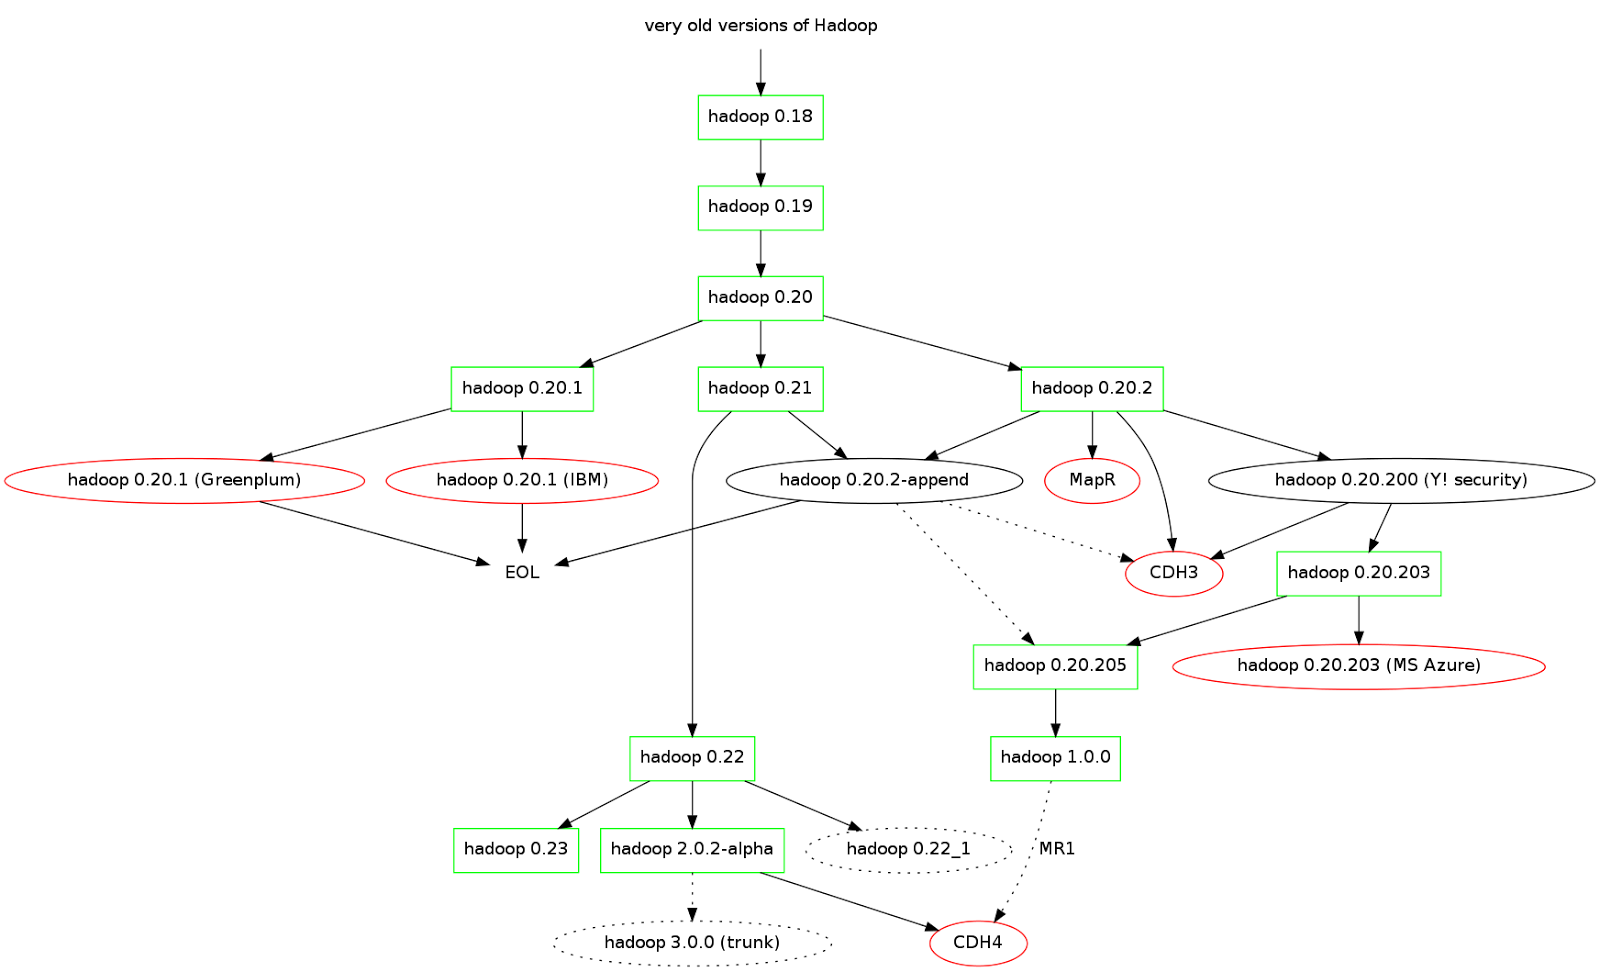
\includegraphics[width=\linewidth]{hadoop_versions.png}
\end{frame}

\begin{frame}{Goals and organization}

\begin{block}{Apache Software Foundation}
Software projects must be cleaned up to be included in Apache (Hadoop branching resulted from competition between Apache clean-up and Cloudera/MapR/IBM/Microsoft feature requests).

\begin{itemize}
\item Non-profit organization.
\item Business-friendly licensing (no ``copyleft'').
\item Individual code contributions are owned by contributors {\it and also} owned by Apache with Apache as copyright holder (\url{http://www.apache.org/legal/src-headers.html}).
\item Presented as a single license with unified header blocks on all source files.
\end{itemize}

Apache includes competing projects that reproduce each other's functionality: \textcolor{darkblue}{Storm}, \textcolor{darkblue}{Spark-Streaming}, \textcolor{darkblue}{S4}, \textcolor{darkblue}{Samza}, \textcolor{darkblue}{Flink} (distributed stream processors).
\end{block}
\end{frame}

\begin{frame}[fragile]{Functional primitives in C++ type syntax}
\small
\begin{verbatim}
iterator<X> filter(iterator<X>, function<bool(X)>);

iterator<Y> map(iterator<X>, function<Y(X)>);

iterator<X> flatten(iterator<list<X>>);

iterator<Y> flatMap(iterator<X>, function<list<Y>(X)>);

Y reduce(iterator<Y>, function<Y(Y,Y)>);

map<K,list<V>> groupByKey(iterator<pair<K,V>>);

map<K,V> reduceByKey(iterator<pair<K,V>>,     // input data
                     function<V(V,V)>);       // merge

map<K,Z> aggregateByKey(iterator<pair<K,V>>,  // input data
                        Z,                    // starting value
                        function<Z(V,Z)>,     // increment
                        function<Z(Z,Z)>);    // combine
\end{verbatim}

%% \vspace{0.5 cm}
%% A standard SQL statement uses three of the above:
%% \begin{verbatim}
%% SELECT <map> FROM source WHERE <filter> GROUP BY <groupByKey>
%% \end{verbatim}

%% \vspace{0.5 cm}
%% Hadoop ``mappers'' are as powerful as {\tt flatMap} and Hadoop ``reducers'' are actually {\tt aggregateByKey}.
\end{frame}

\end{document}
